\chapter{\label{ch:2-bkgnd}Background}

\minitoc

This chapter describes fundamental concepts and gives literature review about research topics that are involved in this thesis. Topics covered include modeling and simulation, co-simualtion, parallel computing, scheduling in the context of parallel computing, and parallelization approaches related to (co-)simulation. 

\section{Modeling and Simulation}

The complex nature of Cyber Physical Systems impose the study of their behavior before building them with the objective of allowing preliminary evaluation, tuning and possibly redesign of the solution. Simulation has proven successful in responding to this need and is becoming an indisputable step in the design process of complex systems. Simulation is an effective cost reducer since it allows to correct design errors before building the system. Simulation is performed by providing models which describe the behavior of the system and then running these models in order to produce the behavior of the simulated system on a computer.   

\subsection{Cyber-Physical Systems}

\subsection{Modeling}

Modeling a system consists in creating a mathematical abstraction of its behavior. The first step is to choose a modeling formalism. This choice depends on the properties of the system, the objective of the simulation, and the aimed level of detail in the simulation. For instance, models can be built using continuous-time variables to represent continuous dynamics of a physical process. Such mathematical models consist of a set of differential equations which describe the continuously changing physical quantities of a process such as electrical circuits, fluid dynamics, chemical reactions, etc. Other systems feature a behavior which evolves between a finite set of states. These systems can be modeled as discrete event systems using formalisms such as DEVS (Discrete Event System Specification), Statecharts, or Petri nets. Finally, hybrid modeling allows the modeling of systems with both continuous variables and discrete states. In other words, the system jumps between discrete states and while it is in a certain state, it features a continuous behavior, i.e. its quantities change continuously. 

In this thesis, we focus on the the modeling of dynamical systems using differential equations. A differential equation expresses a variable as a function of its derivatives. In the modeling of dynamical systems, the variables are the physical quantities and the derivatives express their rates of change. A differential equation is called Ordinary Differential Equation, abbreviated ODE, if it involves ordinary derivatives of the variables with respect to an independent variable (usually the time in the modeling of dynamical systems).  Equation \ref{ode} is an ODE where $x$ is the vector of the dependent variables of interest called the state variables, $\dot{x} = \frac{dx}{dt}$ is the vector of the time derivatives of the state variables, $t$ is the time (the independent parameter), and $f$ is a given function.

\begin{equation}
\dot{x} = f(x,t)
\label{ode}
\end{equation}

In contrast, a differential equation is called Partial Differential Equation, abbreviated PDE if it involves unknown functions and their partial derivatives. Equation \ref{pde} shows such PDE where $x_1,x_2,\dots, x_n$ are the parameters, $y=y(x_1,x_2,\dots, x_n)$ is the unknown function, and $f$ is a given function.

\begin{equation}
f\biggl(x_1,x_2,\dots, x_n,y,\frac{\partial y}{\partial x_1},\frac{\partial y}{\partial x_2},\dots,\frac{\partial y}{\partial x_n}\biggl)=0
\label{pde}
\end{equation} 

In this thesis, we are interested, in particular, in modeling dynamical systems using ODEs.


%Given these equations, the system can be characterized by a number of state variables. The time derivative of each variable is then expressed as a function of the other variables and the inputs. %As a simple example, the fall of a punctual body subject only to gravity can be described by the differential equation:
\subsection{Simulation}

\subsection{Co-simulation}

The following definition is taken from \cite{sicklinger:2014}:

\textit{
In co-simulation the different subsystems which form a coupled problem are modeled and simulated in a segregated manner. Hence, the modeling is done on the subsystem level without having the coupled problem in mind. Furthermore, the coupled simulation is carried out by running the subsystems in a blackbox manner. During the simulation the subsystems will exchange data.}


Co-simulation is an alternative approach to monolithic simulation where a complex system is modeled as a whole using differential equations and simulated by numerically solving these equations. In a CPS, the controlled physical process constitutes a multi-physics system and is modeled in the continuous-time domain using (hybrid) Ordinary Differential Equations (ODEs). Because they are implemented on embedded computers, numerical laws that control the physical process are modeled in the discrete-time domain. All of these features add to the complexity of the numerical models. Co-simulation has a number of advantages over the monolithic approach. It allows modeling each part of the system using the most appropriate tool instead of using a single modeling software. Also, it allows a better intervention of the experts of different fields at the subsystem level. Furthermore, co-simulation facilitates the upgrade, the reuse, and the exchange of models. 

In co-simulation, the equations of each model are integrated using a solver separately. Models exchange data by updating their inputs and outputs according to their communication steps. Figure~\ref{fig:cosim} shows the evolution of time and data exchange between two models. For simplicity, the shown models A and B have identical communication steps $H_A$ and $H_B$ respectively. On the other hand, models A and B have different integration steps $h_A$ and $h_B$ respectively.

\begin{figure}[htb]
\centering
  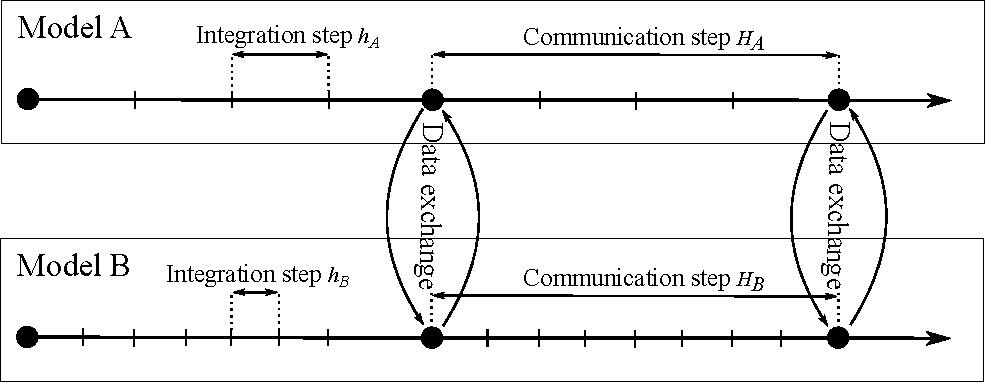
\includegraphics[scale=0.7]{figures/Co-Simulation}
\caption{Evolution of time and data exchange between two models during co-simulation}
\label{fig:cosim}
\end{figure}

\subsection{Co-simulation with Real-time Constraints}

\section{Parallel Computing}

\subsection{Overview}

\subsection{Types of Parallelism}

Different kinds of parallelism exist: bit-level, instruction-level, data, and task parallelism.

\subsubsection{Bit-level parallelism}
Bit-level parallelism is the lowest level of parallelism and is related to the word size of the processor. If a 8-bit processor needs to perform computation on 16-bit data, it has to execute it in at least two steps, first on the 8 lower-order bits of the data and then on the 8 higher-order bits. Increasing the word size of the processor to 16 would allow the computation to be executed in one instruction. 

\subsubsection{Instruction-level parallelism}
Instruction-level parallelism allows the execution of more than one instruction per clock cycle if the instructions do not depend on each other. An example of instruction-level parallelism is instruction pipeline in which an instruction is divided into several steps that can be executed in parallel.

\subsubsection{Data parallelism}
Data parallelism is characterized by performing the same computation on a large set of data. If several processors are available, the data can be distributed across them and the same computation is executed on each processor.  

\subsubsection{Task parallelism}
In task parallelism, a program is divided into different computational tasks that are distributed across the processors to be performed in parallel. The challenge here is the question of how to divide the program efficiently so as to obtain the best speedup.

In contrast to bit-level and instruction-level parallelism, data and task parallelism is apparent to the programmer who should make the decision of how to divide and allocate the data or the tasks of the application. In this thesis, we are interested in particular in task parallelism because the applications that we deal with are more suitable for this kind of parallelism.

\subsection{Types of Parallel Computers}

From a hardware point of view, parallel computers can be classified according to the type of interconnection and communication between the different processors which make up them.

\subsubsection{multicore computing}
A multicore processor contains multiple processing elements, called cores, on the same chip. The different cores can execute instructions simultaneously and thus accelerate the execution time of a program. The different cores are physically close to each other and share the same memory. The computation power of a multi-core processor can be increased by adding more cores. In order to take advantage of multicore processors, appropriate programming paradigms need to be used.  

\subsubsection{Distributed computing}
A distributed computer has several processing elements that are connected by a network and that has each a memory. We talk then of distributed memory.

\subsubsection{Symmetric multiprocessing}
A symmetric multiprocessor computer has several processors that share memory and that are connected by a bus.

\subsubsection{Cluster computing}
A cluster is composed of a number of interconnected optionally heterogeneous computers. If the computers are not identical, balancing the load among the computers becomes difficult.

\subsubsection{Massively parallel computing}
A massively parallel processor (MPP) has a large number of processors, generally more than 128, that are interconnected by means of a network. MPP differ from clusters in that they use specialized networks to connect processors whereas clusters use common networks, e.g. Ethernet, to connect standalone computers.

\subsubsection{Grid computing}
Grid computing is the most distributed kind of parallel computing. A grid uses remote computers connected via the internet.  
 
\subsubsection{General-purpose computing on graphics processing units}
Graphics Processing Units (GPU) are usually used to perform graphics computations on a computer. General-Purpose computing on Graphics Processing Units (GPGPU) consists in using GPUs to perform computing of applications, different than graphics, which are usually executed by Central Processing Units (CPUs). This form of parallel computing  is very efficient for data-parallel applications such as matrix operations.

\subsection{Parallel Programming}

In order to efficiently use parallel computers, many programming approaches have been developed such as libraries, APIs, and programming models. Basically they differ according to the targeted type of memory, i.e. shared memory, distributed memory or shared distributed memory. In a shared memory model, communication is performed by manipulating variables in the shared memory. On the other hand, in a distributed memory model, communication is done by message passing. We present here, one of the most used shared memory libraries (Open Multi-Processing) and one of the most used distributed memory libraries (Message Passing Interface).

\subsubsection{Open Multi-Processing}
Open Multi-Processing (OpenMP) \cite{openmp} is an API that has been designed to develop applications that are meant to be executed on shared memory parallel computers such as multicore computers. OpenMP is supported by C, C++ and Fortran programming languages. The basic idea of OpenMP is that a master thread is responsible for the creation of slave threads that are allocated to processors to run in parallel. The creation of slave threads is called forking. It is the duty of the developer to specify parts of the code that can run in parallel using preprocessor directives. These directives cause the threads to be created before their execution. When the execution of the slave threads is finished, they join back to the master thread which continues the execution of the program. OpenMP can be used for both data and task parallelism.

\subsubsection{Message Passing Interface}
Message Passing Interface (MPI) \cite{mpi} is a standard for programming distributed memory parallel computers. It is based on the concept of message passing between threads that are running in parallel on different processors. It is supported by many programming languages and platforms. It defines a communication protocol for performing the message passing and provides communication and synchronization functionalities for collaborating processes that are allocated to different processing elements. It supports different kinds of communications such as point-to-point and collective communication. It is also possible to choose the topology of communication to be used.

\subsection{Parallel Scheduling}

One of the most important and central topics in the parallel computing field is automatic parallelization of applications. 

%This task can be achieved by the compiler however most parallel programming models are still dominated by explicit parallelism, i.e. the developer specifies the fraction of the code to be parallelized and how it should be parallelized. 
Parallelization consists in the transformation of a sequential program into a multithreaded one in order to be executed on multiple processors. In order to be parallelized, a program needs to be modeled and its general behavior to be known. In general, a model of a program can be made by dividing the program into tasks of computations and defining dependence between them. 
If the number of the tasks is equal to the number of processors, the parallelization of the program can be achieved by allocating each task to a distinct processor. However, this is not always true in practice, i.e. there may be more tasks than processors. In this case multiple tasks may be allocated to one processor and therefore their execution needs to sequentialized.  
Knowing the time needed to execute each task is also important to model the program. Depending on the application, other properties and constraints can be considered. Having a model of the program, the parallelization consists in defining a schedule for the different tasks, i.e. an allocation to a processor and an execution order for each task. Parallel computing has received much interest in the scheduling theory community and many algorithms and models have been proposed to solve the problem of application parallelization.   

Scheduling in the broad sense refers to the theory, algorithms and systems that deal with problems of sequencing and allocating tasks to resources. Scheduling theory has numerous areas of application like manufacturing, transportation, logistics, sports scheduling, and project management. Scheduling is considered to have a crucial role in parallel computing. A significant part of the research carried out in the scheduling theory field treats problems related to scheduling computational tasks on parallel computers. We focus in this section on the state of the art of scheduling from a computing point of view.

In a scheduling problem, the resources are the processors (or cores of a multicore processor) and the tasks are the computation functions of the application to be executed. Resources are traditionally referred to as computers, or sometimes machines, and tasks as jobs. We use the terms processors, to refer to processing elements of a parallel computing system, and tasks to refer to the computational tasks of the application to be executed.

Basically, a scheduling problem is characterized by a set of $n$ tasks $T = \{t_1, t_2, \ldots, tn\}$ and a set of $m$ processors $P = \{p_1, p_2, \ldots, p_m\}$. Scheduling means allocating tasks form $T$ to processors from $P$ with respect to predefined criteria. Scheduling implies also the definition of an execution order for the tasks that are allocated to the same processor. In general, each task has to be allocated to one and only one processor and a processor can execute at most one task at a time. Additional constraints can be added depending on the problem. 

In scheduling problems, processors can be classified based on their speed of execution \cite{davis:2011}:

\begin{itemize}
\item \textit{Heterogeneous}: The execution speed of a task depends on both the processor and the task. Not all tasks may be executed on all processors.
\item \textit{Homogeneous}: The processors are identical. The execution speed of a given task is the same on all processors.
\item \textit{Uniform}: The execution speed of a task depends only on the speed of the processor. A processor of speed 2 will execute all tasks at exactly twice the speed of a processor of speed 1.
\end{itemize}

A schedule is called preemptive if a the execution of a task can be preempted and resumed later. If a schedule is not preemptive, it is called non preemptive. Furthermore, a scheduling algorithm is either dynamic or static. Dynamic scheduling algorithms are used when some information about the tasks are not known before the execution. The scheduling algorithm makes scheduling decisions online as the information becomes available. Static scheduling algorithms can be used when the characteristics of the tasks, such as dependence between them and their execution times, are known before the execution. It is then possible to compute the schedule of the tasks offline.

Scheduling research has been active for over 60 years now and so many methods and algorithms have been proposed to solve different scheduling problems. Different performance measures can be considered such as the makespan objective, the total completion time objective, and the number of late tasks objective \cite{leung:2004}. Makepsan is the time needed by a computer to process a set of tasks. We focus here on the makespan objective because our goal is to accelerate the execution of simulations and thus to minimize the needed execution time.

The sets of tasks are usually described by Directed Acyclic Graphs (DAGs) $G(V,E)$ where each task is represented by a vertex in $V$ and precedence constraints are represented by edges in $V$. A vertex may have one or more incoming edges which connect it with its predecessors and one or more outgoing edges which connect it with its successors. A task cannot start its execution unless all its predecessors have finished the execution. If a vertex has no predecessor it is called an entry or source vertex. A vertex that has no successor is called an exit or sink vertex. The vertices may be weighted by the execution times of the corresponding tasks (see Figure \ref{fig:dagexample}).

%\begin{figure}[h]
%\centering
%\captionsetup{justification=centering}
%\includegraphics[scale=0.9]{figures/dagexample}
%\caption{A DAG representation of a set of tasks $T = \{t_1, t_2, t_3, t_4\}$ with the dependence $t_1 \rightarrow t_2, t_1 \rightarrow t_3, t_2 \rightarrow t_4,$ and $t_3 \rightarrow t_4$}
%\label{fig:dagexample}
%\end{figure} 

In industrial practice, we distinguish between the "functional" and "non functional" specifications. Functional specification consists in defining what has to be done. Mainly, the different functions of the application and the dependence between them are specified. Non functional specification consists in defining how the functions have to be performed. It provides a description of the hardware architecture, its different components and how they are interconnected. It specifies also allocation constraints if there are any and the timing parameters of the different functions, like their execution times and periods.

Having both the functional and non functional specifications, we can deduce the "potential" and the "effective" parallelisms. The potential parallelism is related to the functional specification. It is defined by the functions that are not dependent because they can be executed in parallel, for example $t_2$ and $t_3$ in Figure \ref{fig:dagexample}. The effective parallelism is defined by the hardware architecture, i.e. how many processing elements (processors, cores, \ldots) are able to execute functions in parallel. If the effective parallelism is less or equal to the potential parallelism, the execution of the application is accelerated. If it is greater, the execution is accelerated also but, no matter how much the effective parallelism is increased, the speedup remains constant. In fact, this falls in the scope of Amdahl's law because it describes how hardware parallelism limits the exhibition of the application parallelism.

In the following we review scheduling heuristics that are proposed in the literature for makespan minimization. Heuristics are usually used to solve parallel scheduling problems because these problems are NP-Hard and using exact algorithms results in exponentially increasing execution times.  
In the following we review scheduling heuristics that are proposed in the literature for makespan minimization. Heuristics are usually used to solve parallel scheduling problems because these problems are NP-Hard and using exact algorithms results in exponentially increasing execution times.  

A well-known algorithm in the literature to minimize the makespan of a graph with no transitive arcs is Hu's algorithm \cite{hu:1961}. It assigns a level to each vertex in G as follows: All vertices that have no immediate successor are at level 1. Then for each of the other vertices, the level is equal to one plus the maximum level of its immediate successors. Hu's algorithm proceeds repeatedly by allocating each time the ready task (whose all immediate predecessors have already been allocated) and which has the highest level among all ready tasks to the first available processor. Coffman-Graham algorithm \cite{coffman:1972} performs the scheduling in two steps. First a task is labeled with a label which is a function of the labels of its immediate successors (the labeling algorithm is not detailed here). Tasks are then allocated following a highest label first policy. \cite{papadimitriou:1979} dealt with the problem of scheduling interval-ordered task graphs. In such a graph, two vertices are precedence-related if and only if they can be mapped to non-overlapping intervals on the real line \cite{fishburn:1985}. A task is assigned a priority based on the number of its successors. A list of the tasks is constructed in a descending order of their priorities and then the tasks are assigned in this order. \cite{adam:1974} presents a number of level-based algorithms for scheduling task DAGs among which: The Highest Level First with Estimated Times algorithm labels the vertices of the DAG with levels where the level corresponds to the sum of computation costs on the longest path from the vertex to a sink vertex. It then allocates the tasks in a highest-level first fashion, therefore, the level of a task represents its priority. Highest Levels First with No Estimated Times algorithm works similarly but with the assumption that all tasks have unit computation costs. \cite{kasahara:1984} proposes a similar algorithm with the improvement of breaking ties by selecting the vertex with the largest number of successors. \cite{shirazi:1990} proposes two algorithms: the Heavy Node First algorithm is based on a local analysis of the vertices at each level and allocates the heaviest vertice first. The second algorithm, WL (Weighted Length), considers a global view of the DAG by taking into account the relationships among the nodes at different levels. \cite{kruatrachue:1987} proposed the ISH algorithm. The main idea of ISH is to fill the "scheduling holes"  which are the idle time slots as the schedule is being constructed. The MCP (Modified Critical Path) algorithm proposed by \cite{wu:1990} uses the measure of how late can a task be delayed without increasing the makespan of the schedule. MCP assigns priorities to tasks in an ascending order of their latest start dates. \cite{hwang:1989} Earliest Start Time algorithm computes at each step, for each task, the earliest start date and selects the task that has the smallest one to allocate it. The DLS (Dynamic Level Scheduling) algorithm \cite{sih:1993} assigns dynamic levels to tasks. The dynamic level of a task is equal to the difference between the b-level (longest path from the corresponding vertice to a sink vertice) of the task and its earliest start date. At each step, the algorithm computes the dynamic levels for the ready tasks on all processors. The task-processor pair that gives the largest DL is selected for scheduling. \cite{yang:1994} presents the DSC algorithm which uses an attribute called the dominant sequence which is the critical path of the partially ordered graph.

A current trend in multiprocessor scheduling is to use meta-heuristics such as Genetic Algorithms (GA) \cite{hou:1994, wu:2004, omara:2010}.

\subsection{Parallel Real-time Scheduling}

Real-time scheduling concerns the scheduling of tasks in real-time systems. Here, real-time does not mean fast but it refers to systems that must be able to respond to external events within specified deadlines. Real-time systems are typically found in the form of embedded systems that control physical processes: They represent the cyber part in a CPS. In general, real-time systems are computing systems that are characterized by timing constraints in addition to the functional requirements. A part of this thesis deals with HiL simulation which is a kind of real-time systems because the simulated part has to meet predefined deadlines in order to ensure correct results.
In order to implement real-time applications, first, \textit{real-time tasks} are defined by characterizing the functions obtained from the functional specification by a number of temporal parameters. A real-time task $t_i$ is characterized by the following parameters (Figure \ref{fig:taskmodel}):
\begin{itemize}
\item Release time $r^k_i$: Typical real-time applications consist of a set of tasks that are executed repeatedly where each execution is called an instance. The time at which an instance becomes ready to be executed is called the activation or the release time. $r^k_i$ is the release time of the $k^{th}$ instance of the task $t_i$;
\item First release time: $r^0_i$, called also offset.
\item Start time $s^k_i$: The time at which the $k^{th}$ instance starts its execution $(s^k_i \geq r^k_i)$;
\item Execution time $C_i$: A real-time task has an execution time which cannot be considered to be fixed and may vary from one execution to another. Therefore, a real-time task is characterized by its Worst Case Execution Time (WCET);
\item Finishing time $f^k_i$: The time at which the $k^{th}$ instance finishes its execution;
\item Response time $R^k_i$: The duration between the release time and the finishing time of the $k^{th}$ instance: $R^k_i = f^k_i - r^k_i$;
\item Absolute deadline $d^k_i$: The time at which the $k^{th}$ instance must finish its execution;
\item Relative deadline $D_i$: The duration, starting from the release time, that the task has to finish its execution;
\item Laxity $l^k_i(t)$: Difference between the absolute deadline and the time for which the task has been running $l^k_i=d^k_i-(t+C_i(t))$.
\end{itemize}

\noindent According to how consecutive instances of a task are activated, three kinds of tasks are distinguished:
\begin{itemize}
\item Periodic tasks: The instances of a given task are activated periodically with a known period. A periodic task is characterized by its period $T_i$;
\item Sporadic tasks: The instances of a task are activated by an event and the minimum time between two successive activations is known. A sporadic task is characterized by $T_i$, its minimum arrival time;
\item Aperiodic tasks: The minimum delay between two activations is not known.
\end{itemize} 

\begin{figure}[h]
\centering
\captionsetup{justification=centering}
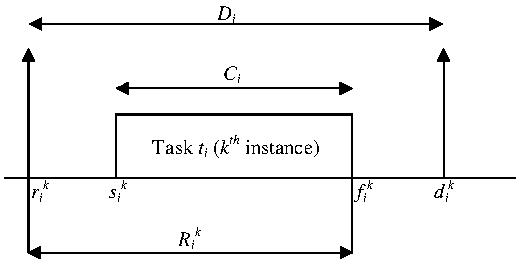
\includegraphics{figures/taskmodel}
\caption{Parameters of a real-time task.}
\label{fig:taskmodel}
\end{figure} 

Real-time systems can be classified based on the impact of missing deadlines. Hard real-time systems are systems where all deadlines must be met. Violating this constraint leads to the failure of the system and may result in a great loss such as serious injuries, threatening human life, or damaging the surroundings. Soft real-time systems can tolerate some deadlines to be missed but the quality of the result degrades consequently. Firm real-time systems allow few deadlines to be missed but if a task's deadline is missed, its result is no more useful. We consider that HiL simulation falls within the category of firm real-time systems. In fact, in order to have correct HiL results, deadlines must be met. If a task misses its deadline, it produces erroneous results and probably causes the failure of the system but the consequences are not as catastrophic and harming as in the case of hard real-time systems.   

Many different real-time scheduling algorithms have been proposed in the literature but they are all based on the same idea, tasks are assigned priorities and then scheduled in an order following their priorities. We distinguish between fixed priorities which do not change during the execution and dynamic priorities which may be changed by the scheduler during the execution. Also, as in other kinds of scheduling problems, real-time scheduling algorithms can be classified into offline/online and preemptive/non preemptive algorithms.

The main goal of scheduling in real-time systems is to satisfy the different timing constraints of the tasks. Schedulability tests are performed to check whether the tasks can be scheduled using a given scheduling algorithm in such a way to satisfy all the requirements. The schedulability test verifies if the utilization or the density of the processor, defined below, when it executes the set of tasks under test, is within a least upper bound. For a set of $n$ independent periodic tasks, the utilization factor and density, when a preemptive scheduling algorithm is used, are respectively:

\begin{equation}
U = \sum_{i=1}^{n}\frac{C_i}{T_i}
\end{equation}

\begin{equation}
\Delta = \sum_{i=1}^{n}\frac{C_i}{D_i}
\end{equation}
The most known real-time scheduling algorithms are the following:

\begin{itemize}
\item Fixed priorities
\begin{itemize}
\item Rate Monotonic (RM): Tasks are assigned priorities inversely proportional to their periods. A set of tasks is schedulable by RM if: $U \leq n(2^{\frac{1}{n}}-1)$, $D_i = T_i$. 
\item Deadline Monotonic (DM): Tasks are assigned priorities inversely proportional to their relative deadlines. Tasks are schedulable using DM if: $\Delta \leq n(2^{\frac{1}{n}}-1)$, $D_i \leq T_i$. 
\end{itemize}
\item Dynamic priorities
\begin{itemize}
\item Earliest Deadline First (EDF): Priorities of tasks are inversely proportional to their absolute deadlines. The priority of a task is fixed for one instance but may change from one instance to another. EDF can schedule a set of tasks if and only if: $U \leq 1, D_i = T_i$.
\item Least Laxity First (LLF): Priorities of tasks are inversely proportional to their laxities. The priority may change for the same instance and from one instance to another. The schedulability test is the same as for EDF.
\end{itemize}
\end{itemize}
 For multiprocessor real-time scheduling, there exist two principal approaches:

\begin{itemize}
\item Global scheduling: Each task can be scheduled on any processor. the scheduler is responsible for migrating the tasks between the processors.
\item Partitioned scheduling: The tasks are partitioned into groups, each of which is allocated to one processor. Each processor has a single-processor scheduler. 
\end{itemize}
Global multiprocessor scheduling has significant overhead due to the migration cost. That is the reason why partitioned scheduling is usually used in hard real-time systems. Partitioning and allocating a set of tasks is equivalent to the "Bin Packing" problem which is NP-hard and heuristics are therefore used. 

Assuming the tasks are sorted in a list and that processors are organized in a certain order, the most known heuristics that can be used to allocate a set of tasks to multiple processors are:

\begin{itemize}
\item First Fit (FF): A task is tested on all cores and for each task the test starts from the first core. The task is allocated to the first found core that can schedule it. A task is schedulable on a given core if by allocating it to this core the condition $(U\leq1)$ is valid where $U$ is the utilization of the core.
\item Next Fit (NF): Similar to FF but the search of the core that can schedule the task does not start always from the first one. After allocating a task to a core, the core search for the next task starts from the next core.
\item Best Fit (BF): Test the task on all cores and allocate it to the one that gives the minimum of $U$.
\item Worst Fit (WF): Allocate the task to the core that gives the maximum of $U$.
\end{itemize}
  
\section{Parallelization of Co-simulation}

In this section we briefly review some of the approaches in the literature on the parallelization of simulations. We present also some of the available simulation tools that support parallel simulations.

\subsection{Methods}

In order to achieve simulation acceleration using multicore execution, different approaches are possible and were already explored. Some approaches seek to parallelize the integration methods, for example a multi-satge solver requires several computations within one integration step. It is then possible to perform multiple computations in parallel within one step \cite{iserles:1990}. Another approach consists in parallelizing operations on vectors for ODEs resolution like in the PVODE solver \cite{byrne:1999} implemented using MPI. It is possible to modify the model in order to prepare its multicore execution, for example by using marked functions as in \cite{elmqvist:2015,Gebremedhin2012}. If providing OpenMP ready libraries is possible, the key feature for simulation acceleration is to provide techniques which offer speedup whatever the model is. Proposing parallel solvers or automatic parallel executions of model equations as in \cite{elmqvist:2014} is also an efficient approach. \cite{clauberg:2012} presents an approach for the parallelization of simulations on shared memory multiprocessors using OpenMP to parallelize matrix operations. Transmission Line Modeling \cite{hui:1990} is a method that allows the decoupling and the parallelization of models by representing them using transmissionline graphs such that decoupling points are chosen where variables change slowly because the models are considered as if they were connected by constants at these points. \cite{sjolund:2010,braun:2012} are based on the TLM method. As shown in \cite{Benkhaled_A_2012_ECOSM}, splitting a model into several FMUs, by isolating discontinuities, may reduce the simulation time, even in the case of a monocore execution. \cite{benkhaled:2014} presents the RCOSIM approach. It consists in using each FMU information on input/output causality to build a graph, with an increased granularity and then exploiting the potential parallelism by using a heuristic to build an offline multicore schedule.

\subsection{Tools}

In this section, we present some of the available simulation tools that support parallel execution.

\subsubsection{xMOD}
xMOD\footnote{http://www.xmodsoftware.com/} is the modeling and simulation software developed by IFP Energies nouvelles. It supports FMI and provides an environment for the integration of heterogeneous models built by different parties using different languages and tools. xMOD can execute models embedding different solvers with different step-times on multicore architectures enabling the acceleration of complex simulations execution. The parallelization approach of xMOD is based on scheduling graphs of tasks. The approach is detailed in chapter \ref{methods}. Figure \ref{fig:mips} shows an example of co-simulation models connected in xMOD. 

%\begin{figure}[h]
%\centering
%\captionsetup{justification=centering}
%\includegraphics[scale=0.5]{figures/mipsxmod}
%\caption{Example of co-simulation models in xMOD.} 
%\label{fig:mips}
%\end{figure} 

\subsubsection{MATLAB Simulink}
Simulink\footnote{www.mathworks.com/products/simulink/}, developed by Mathworks is a graphical modeling environment. It is intended to simulate dynamical systems that can be described using block diagrams. Simulink allows parallel execution by allowing the partitioning of the models and allocating them to a multicore processor in such a way to balance the computational load. The user can configure the parallelization using a graphical interface.

\subsubsection{Dymola}
Dymola\footnote{http://www.3ds.com/products-services/catia/products/dymola}, developed by Dassault Syst\`emes AB, is a modeling and simulation environnement based on the open Modelica modeling language. Dymola can parallelize the computations of model equations. It finds which equations can be be parallelized and automatically introduces OpenMP directives. The parallelization process is detailed in \cite{elmqvist:2014}.

\subsubsection{Amesim}
Amesim\footnote{www.plm.automation.siemens.com/en\_us/products/lms/imagine-lab/amesim/} is a modeling and simulation software developed by Siemens PLM Software. Amesim allows launching multiple simulations in parallel, for example to run a model with different parameters. It has also the capability of partitioning models and executing them on multicore processors.

\subsubsection{Hopsan}
Hopsan\footnote{https://www.iei.liu.se/flumes/system-simulation/hopsan?l=en} is a free multi-domain system simulation tool developed at the division of Fluid and Mechatronic Systems at Link\"oping university. The parallelization approach of Hopsan is based on the TLM method \cite{sjolund:2010,braun:2012}.

\subsubsection{MBSim}
MBSim\footnote{https://github.com/mbsim-env/} is a simulation environment for multibody systems developed at the Institute of Applied Mechanics of the Technische Universit\"at M\"unchen. It is able to run simulations on multicore processors by using OpenMP library to parallelize matrix operations \cite{clauberg:2012}.    